\documentclass{report}
\usepackage[utf8]{inputenc}
\usepackage{hyperref}
\usepackage{setspace}
\usepackage{float}
\title{Universal Parabolic Constant}

\author{Balakrishnan Rajagopal (40075977) }
\date{}
\renewcommand{\baselinestretch}{1.15}

\usepackage{natbib}
\usepackage{graphicx}

\usepackage[final]{pdfpages}


\usepackage{fancyhdr}
\usepackage[margin=1in]{geometry}
\usepackage{pdfpages}
\renewcommand{\headrulewidth}{0.1pt}
\fancyhf{} 
\renewcommand{\headrulewidth}{0.1pt} 
\fancyfoot[C]{\thepage} 
\renewcommand{\footrulewidth}{0.1pt} 


\begin{document}
\maketitle
\chapter{Universal Parabolic Constant}
\section{Description}
\onehalfspacing
The Universal parabolic constant is a mathematical constant and is defined as the ratio, for any parabola, of the arc length of the parabolic segment formed by the latus rectum to the focal parameter. The focal parameter is twice the focal length. The ratio is denoted P. Just as the ratio of the arc length of a semicircle to its radius is always pi, the ratio P of the arc length of the parabolic segment formed by the latus rectum of any parabola to its semilatus rectum (and focal parameter) is a universal constant. The other conic sections, namely the ellipse and hyperbola, do not have such universal constants because the analogous ratios for them depend on their eccentricities. In other words, all circles are similar and all parabolas are similar, but the same is not true for ellipses or hyperbolas.\newline
\newline The value of P is,

\begin{equation}
P = \ln(1+\sqrt{2})+\sqrt{2} = 2.29558714939
\end{equation}

\newline In the diagram (Fig 1), the latus rectum is pictured in blue, the parabolic segment that it forms in red
and the focal parameter in green. (The focus of the parabola is the point F and the directrix is the line L.)



\begin{figure}
\centering
    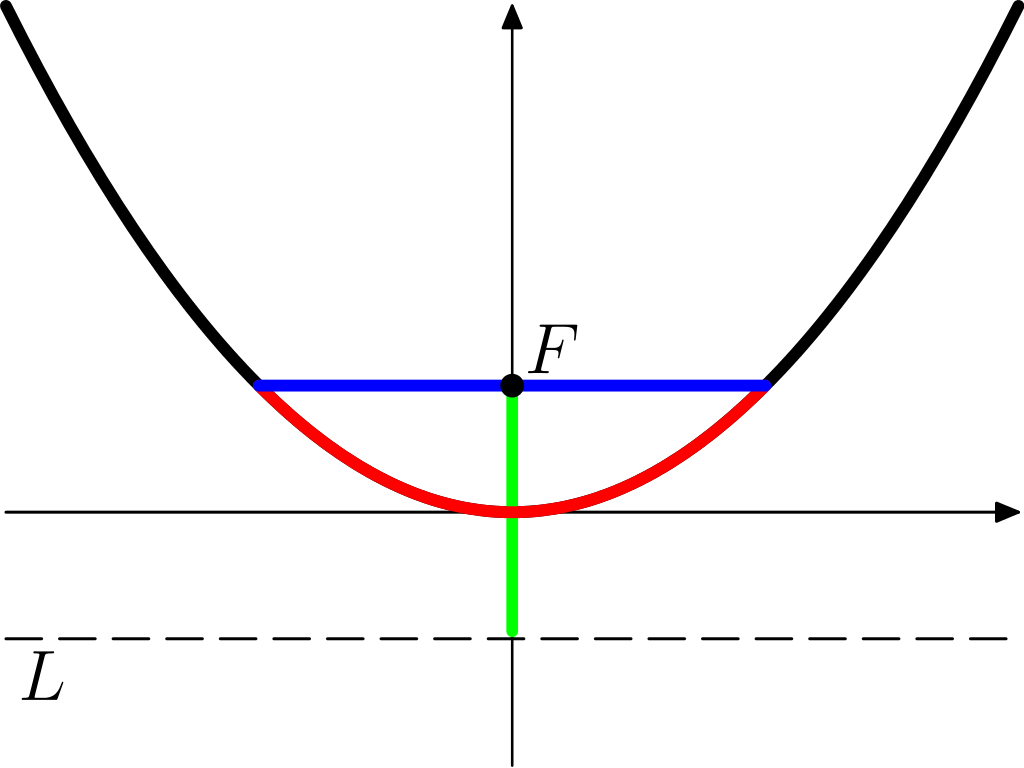
\includegraphics[width=.2\textwidth,center]{upc.png}
    \caption{The universal parabolic constant is the red length divided by the green length.}
\end{figure}

\section{Properties}
\onehalfspacing
\newline
\begin{itemize}
  \item P is an irrational number.
  \item It is also a transcendental number.
\end{itemize}







\bibliographystyle{plain}
\bibliography{references}
\end{document}